\subsection{Graph}
\begin{frame}[fragile]
\frametitle{Graph}
{\small
A graph data structure consists of a finite set of nodes and connections.
These connections are known as edges in an undirected graph and as arrows in a directed graph.
In the following graph, each node has a value and each edge has a weight.\\
\vspace{3mm}
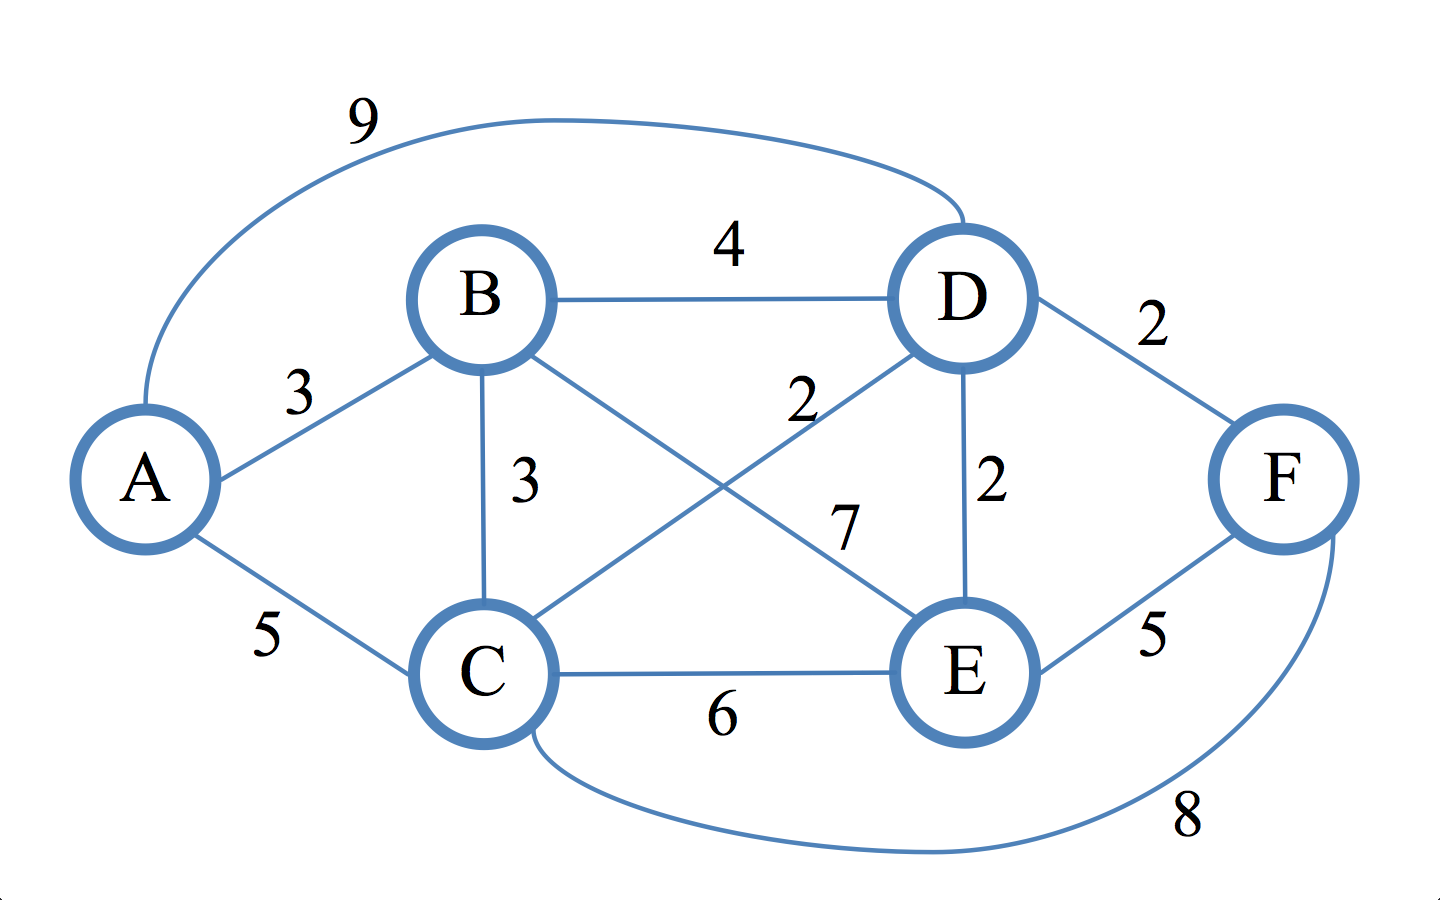
\includegraphics[scale=0.08]{img/graph.png}\\
\vspace{3mm}
Graph algorithms are a significant field of interest within computer science. Typical higher-level operations associated with graphs are:
finding a path between two nodes, like depth-first search and breadth-first search and finding the shortest path from one node to another.
}
\end{frame}

\begin{frame}[fragile]
\frametitle{Graph}
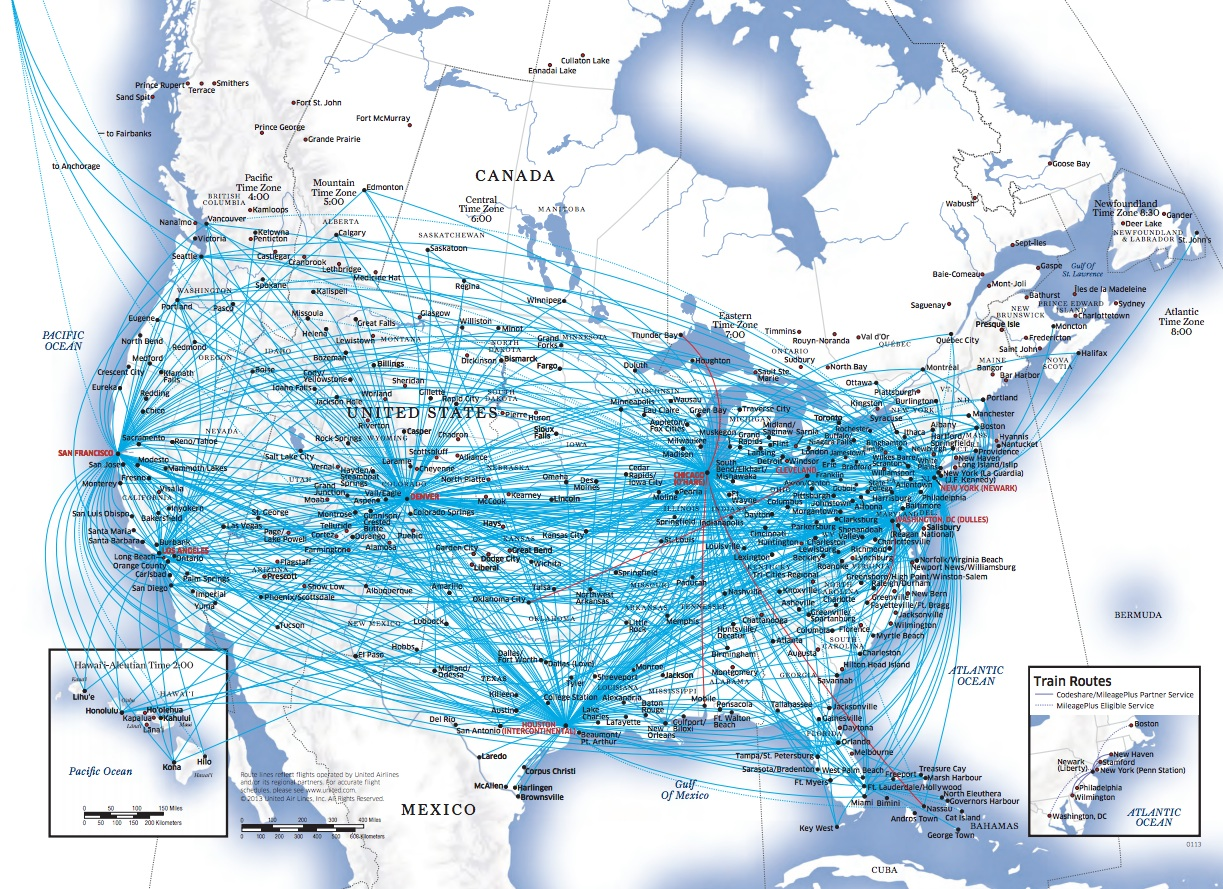
\includegraphics[scale=0.22]{img/flight.jpg}
\end{frame}

\begin{frame}[fragile]
\frametitle{Graph Representation - Adjacency Matrix}
Adjacency Matrix is a 2D array of size \verb|#Nodes x #Nodes|.\\
\vspace{3mm}
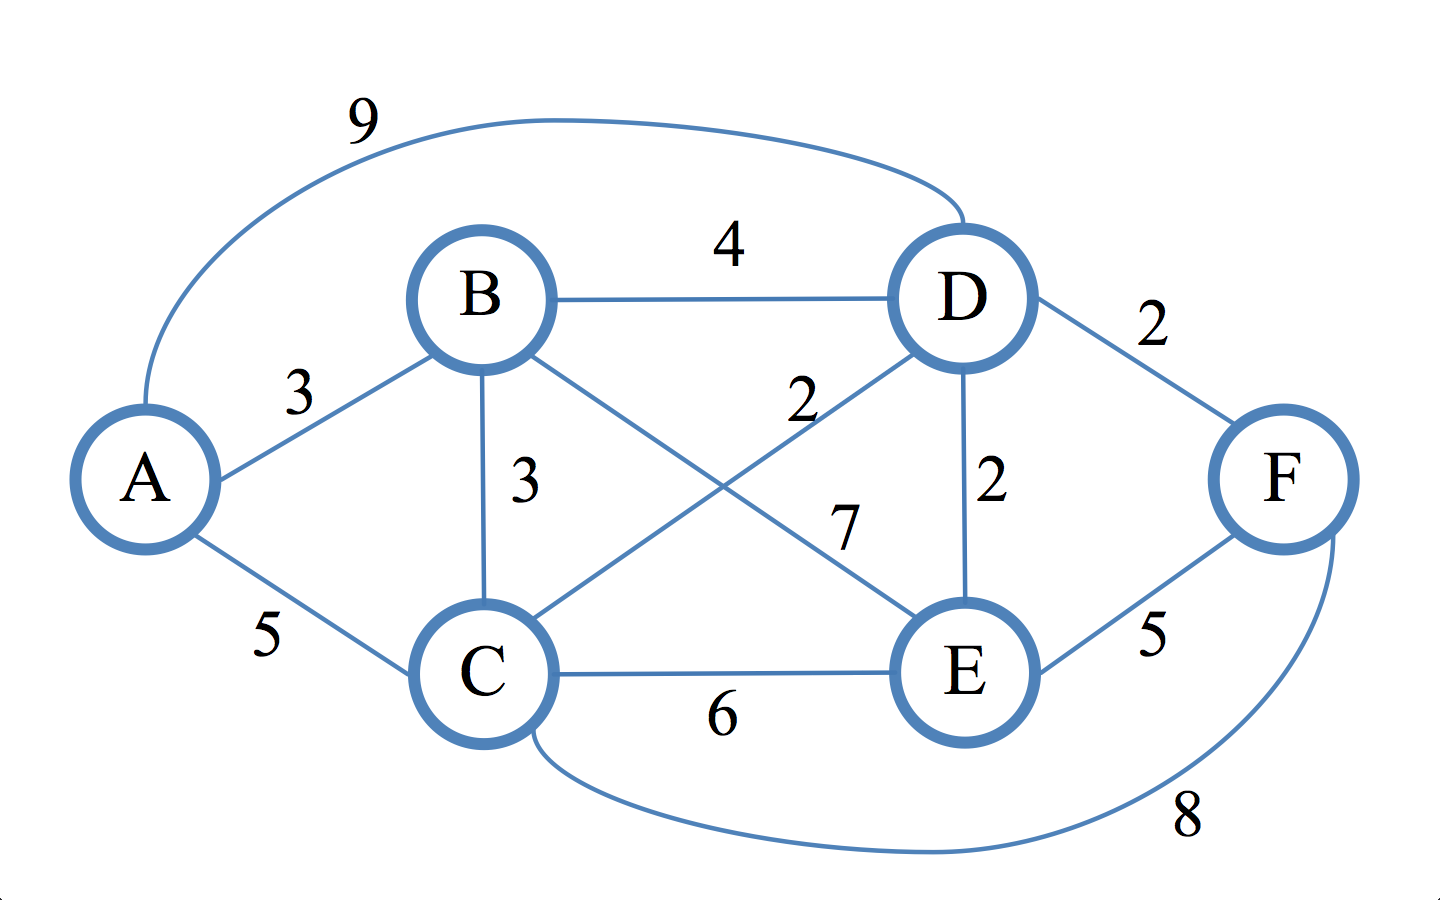
\includegraphics[scale=0.08]{img/graph.png}\\
\vspace{3mm}
\begin{lstlisting}
  A  B  C  D  E  F
A 0  3  5  9  -  -
B 3  0  3  4  7  -  
C 5  3  0  2  6  8
D 9  4  2  0  2  2
E -  7  6  2  0  5
F -  -  8  2  5  0
\end{lstlisting}
\end{frame}

\begin{frame}[fragile]
\frametitle{Graph Representation - Adjacency List}
Adjacency List is an array of list objects.\\
\vspace{3mm}
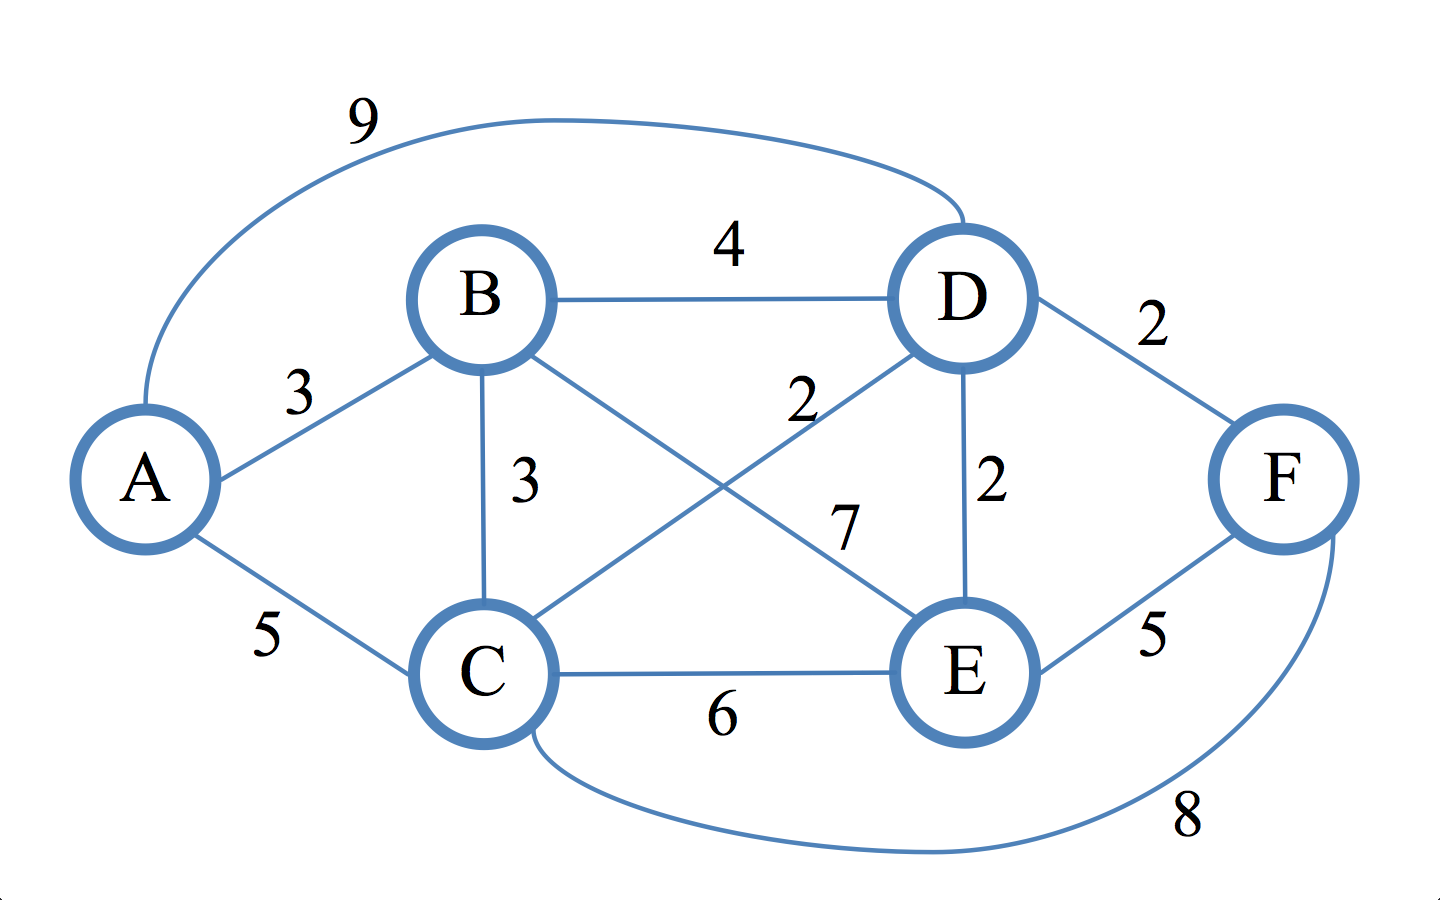
\includegraphics[scale=0.08]{img/graph.png}\\
\vspace{3mm}
\begin{lstlisting}
A {B, C, D}           A {3, 5, 9}
B {A, C, D, E}        B {3, 3, 4, 7}
C {A, B, D, E, F}     C {5, 3, 2, 6, 8}
D {A, B, C, E, F}     D {9, 4, 2, 2, 2}
E {B, C, D, F}        E {7, 6, 2, 5}
F {C, D, E}           F {8, 2, 5}
\end{lstlisting}
\end{frame}

\begin{frame}[fragile]
\frametitle{Graph Representation - Adjacency List}
\begin{exercise}
Create the Graph for the given data:\\
{\tiny
\begin{lstlisting}
Node 0	2(10), 6(14), 9(2), 
Node 1	2(20), 8(5), 9(18), 
Node 2	0(10), 1(20), 3(16), 6(11), 7(14), 8(7), 9(12), 
Node 3	2(16), 5(17), 6(14), 
Node 4	
Node 5	3(17), 7(11), 
Node 6	0(14), 2(11), 3(14), 
Node 7	2(14), 5(11), 9(8), 
Node 8	1(5), 2(7), 
Node 9	0(2), 1(18), 2(12), 7(8),
\end{lstlisting}
}
\end{exercise}
\end{frame}

\begin{frame}[fragile]
\frametitle{Breath First Search}
Breadth-first search (BFS) is an algorithm for traversing a graph data structure. It starts at the tree root and explores the neighbor nodes first, before moving to the next level neighbours.\\
\vspace{3mm}
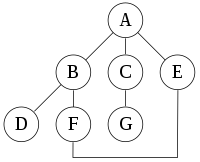
\includegraphics[scale=0.5]{img/graph2.png}\\
\vspace{3mm}
{\bf BFS: A, B, C, E, D, F, G}
\end{frame}

\begin{frame}[fragile]
\frametitle{Depth First Search}
Depth-first search (DFS) is an algorithm for traversing a graph data structure. One starts at the root and explores as far as possible along each branch before backtracking.\\
\vspace{3mm}
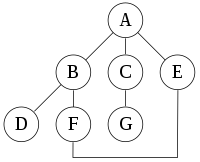
\includegraphics[scale=0.5]{img/graph2.png}\\
\vspace{3mm}
{\bf DFS: A, B, D, F, E, C, G}
\end{frame}

\begin{frame}[fragile]
\frametitle{Dijkstra's Algorithm}
The Dijkstra Algorithm is used to find the shortest path within a weighted graph.\\
The algorithm contains the following steps:

{\tiny
\begin{enumerate}
\item Create a table with 4 columns: Node ID, Distance, Marked, Predecessor.
\item Enter a row for each node into the table and initialize the values:
\begin{itemize}
\item Node ID: The id of the node
\item Distance: $\infty$
\item Marked: \verb|FALSE|
\item Predecessor: $-1$
\end{itemize}
\item Set the distance (0) and the predecessor of the start node.
\item Repeat for all not marked nodes:
\begin{itemize}
\item Search the node X with minimum distance
\item Caclulate the distance from X to all the neighbours\\
Total Cost = CurrentCost at Node X + Weight to the neighbour
\item Check the current table entries. Update the table, if
the distance to a neighbour is smaller.
\end{itemize}
\end{enumerate}
}

\end{frame}

\begin{frame}[fragile]
\frametitle{Dijkstra's Algorithm - Example}
Find the shortest path between a and e.\\
\vspace{3mm}
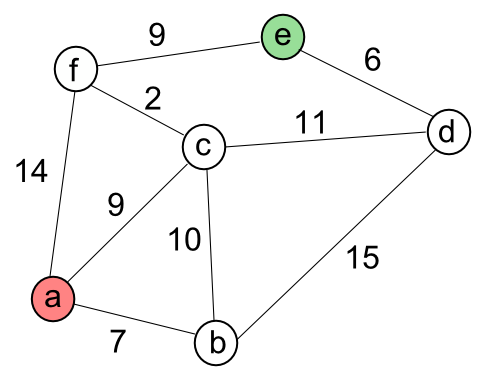
\includegraphics[scale=0.2]{img/dijkstra.png}
\vspace{3mm}
{\tiny
\begin{tabular}{l|l|l|l}
Node ID & Distance & Marked & Predecessor\\
\hline
a & $\infty$ & & -\\
b & $\infty$ & & -\\
c & $\infty$ & & -\\
d & $\infty$ & & -\\
e & $\infty$ & & -\\
f & $\infty$ & & -\\
\end{tabular}
}
\end{frame}

\begin{frame}[fragile]
\frametitle{Dijkstra's Algorithm - Example}
{\tiny
\begin{tabular}{l|l|l|l}
Node ID & Distance & Marked & Predecessor\\
\hline
a & $0$ & & a\\
b & $\infty$ & & -\\
c & $\infty$ & & -\\
d & $\infty$ & & -\\
e & $\infty$ & & -\\
f & $\infty$ & & -\\
\end{tabular}
\begin{tabular}{l|l|l|l}
Node ID & Distance & Marked & Predecessor\\
\hline
a & $0$ & x & a\\
b & $7$ & & a\\
c & $9$ & & a\\
d & $\infty$ & & -\\
e & $\infty$ & & -\\
f & $14$ & & a\\
\end{tabular}
\newline
\vspace{4mm}
\begin{tabular}{l|l|l|l}
Node ID & Distance & Marked & Predecessor\\
\hline
a & $0$ & x & a\\
b & $7$ & x & a\\
c & $9$ & & a\\
d & $22$ & & b\\
e & $\infty$ & & -\\
f & $14$ & & a\\
\end{tabular}
\begin{tabular}{l|l|l|l}
Node ID & Distance & Marked & Predecessor\\
\hline
a & $0$ & x & a\\
b & $7$ & x & a\\
c & $9$ & x & a\\
d & $20$ & & c\\
e & $\infty$ & & -\\
f & $11$ & & c\\
\end{tabular}
\newline
\vspace{4mm}
\begin{tabular}{l|l|l|l}
Node ID & Distance & Marked & Predecessor\\
\hline
a & $0$ & x & a\\
b & $7$ & x & a\\
c & $9$ & x & a\\
d & $20$ & & c\\
e & $20$ & & f\\
f & $11$ & x & c\\
\end{tabular}
\begin{tabular}{l|l|l|l}
Node ID & Distance & Marked & Predecessor\\
\hline
a & $0$ & x & a\\
b & $7$ & x & a\\
c & $9$ & x & a\\
d & $20$ & x & c\\
e & $20$ & x & f\\
f & $11$ & x & c\\
\end{tabular}
}
\end{frame}


